\emph{1. Способы задания движения материальной точки. Векторный и координатный
способы задания движения. Определение траектории движения, скорости, ускорения.}

\vspace*{1em}
Существует три способа задания движения точки: естественный, векторный и
координатный. Остановимся на двух последних.

\header{Векторный способ задания движения}
\begin{table}[h!]
    \begin{tabular}{C{.4}m{.55\textwidth}}
        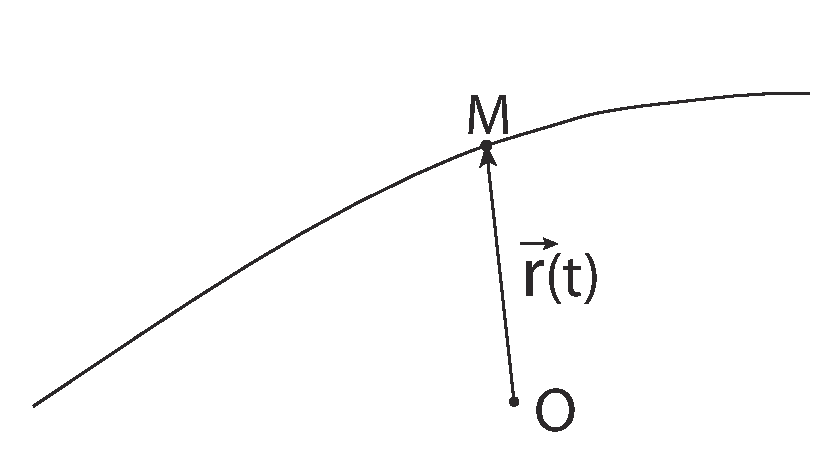
\includegraphics[width=.4\textwidth]{1_vect} &
        Положение точки в пространстве однозначно определяется заданием
        радиус-вектора \( \vec{r} \), проведенного из некоторого неподвижного
        центра \( O \) в данную точку \( M \).
        
        Для определения движения точки нужно знать как меняется с течением
        времени радиус-вектор \( \vec{r} \), то есть должна быть задана
        вектор-функция
    \end{tabular}
\end{table}

аргумента \( t \):
\[
    \vec{r} = \vec{r}(t).
\]

Траектория движения представляет собой геометрическое место концов
радиус-вектора \( \vec{r} \) движущейся точки.

\header{Координатный способ задания движения}

Рассмотрим движение точки \( M \) в трехмерном пространстве. Введем
прямоугольные декартовы координаты \( Oxyz \). Тогда в системе отсчета
\( Oxyz \) положение точки \( M \) определяется тремя координатами
\( (x, y, z) \). При движении точки \( M \) ее координаты изменяются с течением
времени. Следовательно:
\[ \left\{ \begin{array}{l}
    x = f_1(t); \\
    y = f_2(t); \\
    z = f_3(t).
\end{array} \right. \]

Эти уравнения называются уравнениями движения точки в декартовых координатах. Их
можно рассматривать как параметрические уравнения траектории точки. При
исключении параметра \( t \) из уравнений движения получаются уравнения
траектории в координатной форме.

Так, решив первое уравнение относительно \( t \), получим \( t = \phi(x) \).
Подставив полученное выражение для \( t \) в два других уравнения, получаем
уравнения траектории точки в координатной форме:
\[ \left\{ \begin{array}{l}
    x = f_1[\phi(x)]; \\
    y = f_2[\phi(x)].
\end{array} \right. \]
Координатный способ может быть получен из векторного проецированием на орты, так
как имеет место представление радиус-вектора:
\[
    \vec{r}(t) = x(t)\cdot\vec{e}_x + y(t)\cdot\vec{e}_y + z(t)\cdot\vec{e}_z.
\]

\header{Скорость}

Скорость -- это векторная величина, характеризующая быстроту и направление
движения точки в данной системе отсчета. При векторном способе задания движения
скорость:
\[
    \vec{v} \defeq \lim_{\D t \to 0} \Der{\vec{r}}{t} = \der{\vec{r}}{t}.
\]

Из определения следует, что скорость является производной по времени от радиус
вектора и направлена по касательной к траектории в сторону движения точки.

Для координатного способа получим (в декартовых координатах):
\[
    \vec{v} = \der{\vec{r}}{t} = \der{}{t}\Big(x(t)\cdot\vec{e}_x +
    y(t)\cdot\vec{e}_y + z(t)\cdot\vec{e}_z\Big) = \der{x}{t}\cdot\vec{e}_x +
    \der{y}{t}\cdot\vec{e}_y + \der{z}{t}\cdot\vec{e}_z = v_x\cdot\vec{e}_x +
    v_y\cdot\vec{e}_y + v_z\cdot\vec{e}_z.
\]

Следовательно, проекции скорости точки на неподвижные оси декартовых координат
равны первым производным от соответствующих координат точки по времени.

Модуль скорости и её направление можно определить, зная проекции:
\[
    v = \sqrt{v_x^2 + v_y^2 + v_z^2}, \quad
    \cos\left(\vec{v}, \vec{e}_x\right) = \frac{v_x}{v},\ \ 
    \cos\left(\vec{v}, \vec{e}_y\right) = \frac{v_y}{v},\ \ 
    \cos\left(\vec{v}, \vec{e}_z\right) = \frac{v_z}{v}.
\]

\header{Ускорение}

При неравномерном криволинейном движении точки изменяются модуль и направление
её скорости. Ускорение точки характеризует быстроту изменения модуля и
направления скорости точки.
\[
    \vec{a} \defeq \lim_{\D t \to 0} \Der{\vec{v}}{t} = \der{\vec{v}}{t} =
    \dder{\vec{r}}{t}.
\]

Вектор ускорения направлен по касательной к годографу скорости, расположен в
соприкасающейся плоскости и направле в сторону вогнутости кривой.

Как и в случае со скоростью, можно перейти к координатам. Получим:
\begin{align*}
    a_x = \dder{x}{t},\ \ a_y & = \dder{y}{t},\ \ a_z = \dder{z}{t}; \\
    a = \sqrt{a_x^2 + a_y^2 + a_z^2}, \quad
    \cos\left(\vec{a}, \vec{e}_x\right) = \frac{a_x}{a}, & \ \ 
    \cos\left(\vec{a}, \vec{e}_y\right) = \frac{a_y}{a},\ \ 
    \cos\left(\vec{a}, \vec{e}_z\right) = \frac{a_z}{a}.
\end{align*}

\newpage % ---------------------------------------------------------------------
